\begin{bibunit}[IEEEtran.bst]

\chapter{Introduction}
\addcontentsline{toc}{chapter}{Introduction}
\chaptermark{Introduction}




  \section{Broad Context}


In the context of an evolving climate, monitoring the changes in our environment is a critical aspect of our ability to react and adapt.
The oceans are physical systems ruled by known but chaotic dynamics which makes the use of observational data essential to monitor their state.
Our monitoring ability thus depends on the observing systems deployed as well as our ability to exploit the observation data.

In recent decades, satellite NADIR altimeters have greatly improved our observational capabilities by providing a global coverage of the Sea Surface height (SSH).
  However due to the scarce and irregular sampling of altimeter constellations, current operational products provide limited insights into phenomena with time scales of a few days and spatial scales of tens of kilometers\cite{ballarottaResolutionsOceanAltimetry2019}. Figure \ref{fig:ocean_processes} shows the approximate scales of the processes of interest in altimetry and the limit of observational capabilities with the data of a nadir altimeter.
% These processes linked to the mesoscale and submesoscale dynamics of the ocean surface play an important role in the heat redistribution within the ocean, which has implications for climate monitoring.
  This thesis is situated within the context of the Surface Water Ocean topography (SWOT)\cite{KaRInSWOTCharacteristics} mission, which presents opportunities for enhancing our observational capabilities of the oceans. Figure \ref{fig:ssh_intro} shows an simulated example to illustrate the impact of the SWOT mission.
The Ka-band Radar Interferometer (KaRIn) sensor which will provide the depicted two dimensional images of the ocean surface topography but will also introduce calibration challenges\cite{EmpiricalCrossCalibrationCoherent} due to previously unseen errors.


\begin{figure}[H]
\centering    
  % \makebox[\textwidth][c]{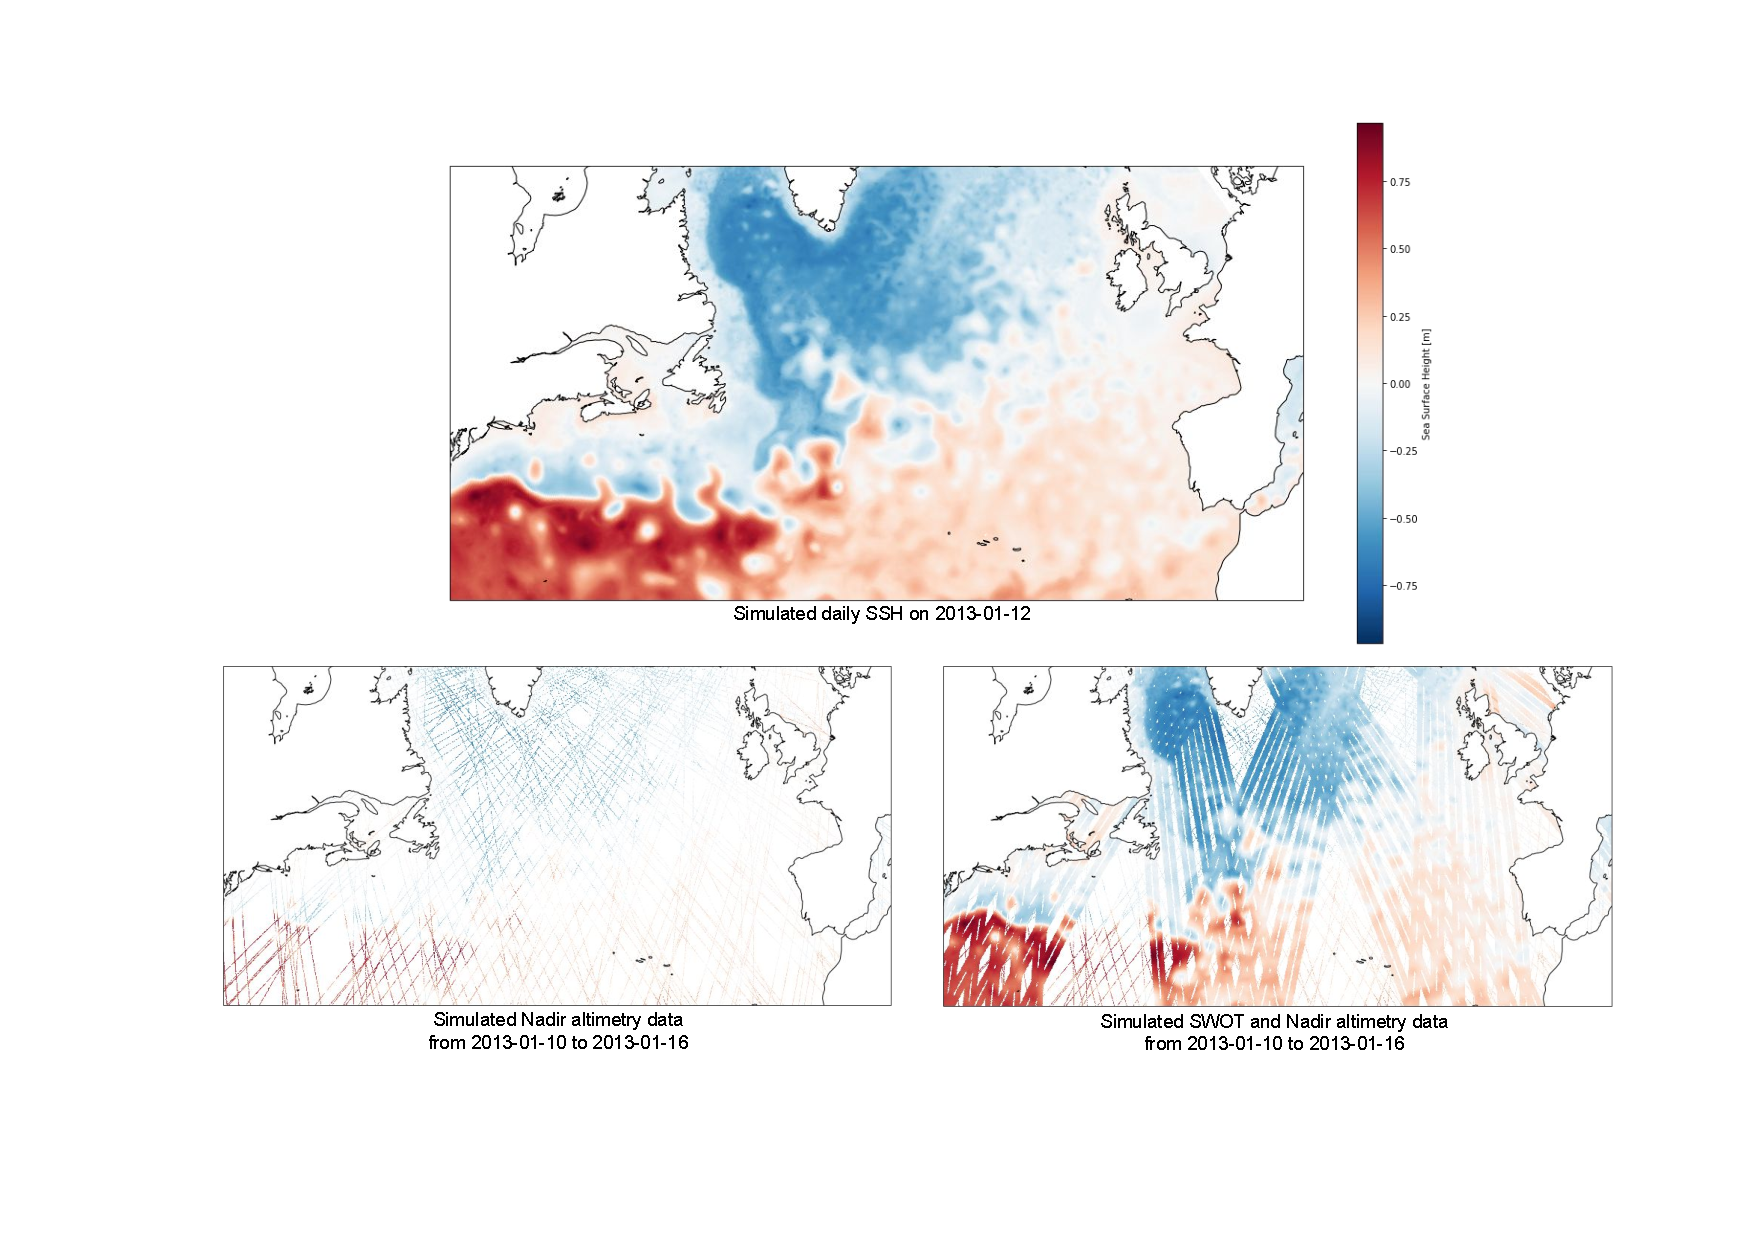
\includegraphics[width=19cm]{Introduction/SSH_intro.pdf}}%
  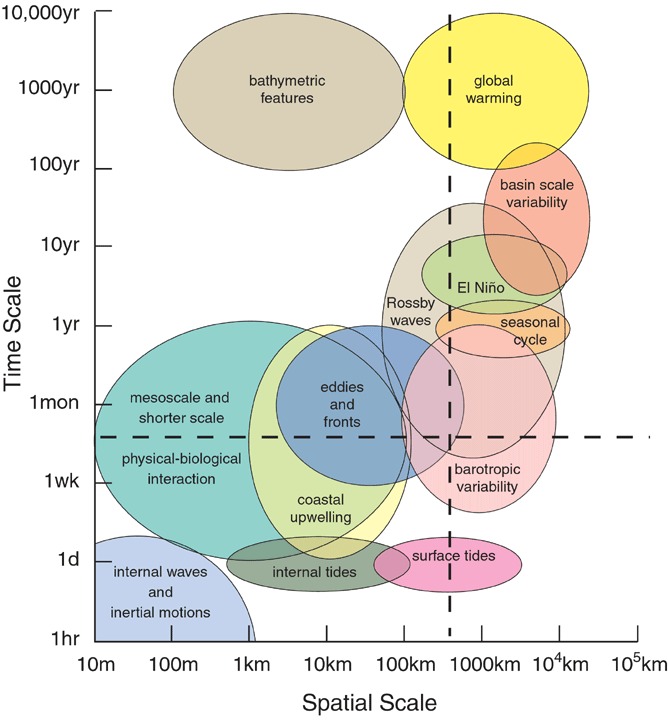
\includegraphics[width=12cm]{Introduction/web_space_time_scales.png}%

    
    \caption{\textbf{Scales of Ocean Processes.} Credits to Dudley B. Chelton. Illustration of the variety of processes of interest for altimetry displayed in function of their spatial and temporal scales. The dashed lines indicate the observational limitations when using a single altimeter data. (Observed phenomena in the top-right section) }
    \label{fig:ocean_processes}
\end{figure}

  The research in this thesis focuses on the development of methods to exploit satellite SSH observations for improving our knowledge of ocean surface dynamics. 
  More specifically we're asking how advances in deep learning can be beneficial to ocean altimetry analysis.
  Deep learning research provides a rapidly evolving set of tools that have been successfully applied to a wide range of domain, surpassing existing methods and succeeding in previously unsolved problems.

  
  In order to study the potentials of deep learning for tackling ocean observation problems, we'll first introduce the necessary methodological components involved when addressing an observation problem by walking through the illustrative example of a thermometer graduation procedure.
  We will explicit the similarities between this example and the altimetry challenges studied in this thesis.
 This simplified problem will help illustrate and contextualize the complementary roles of data and domain knowledge when addressing this class of problem. 
  We will then describe how the tools brought by the deep learning field fit in this methodological framework and consider the opportunities and challenges that arise when applying them to ocean altimetry analysis.


\begin{figure}[h]

  \makebox[\textwidth][c]{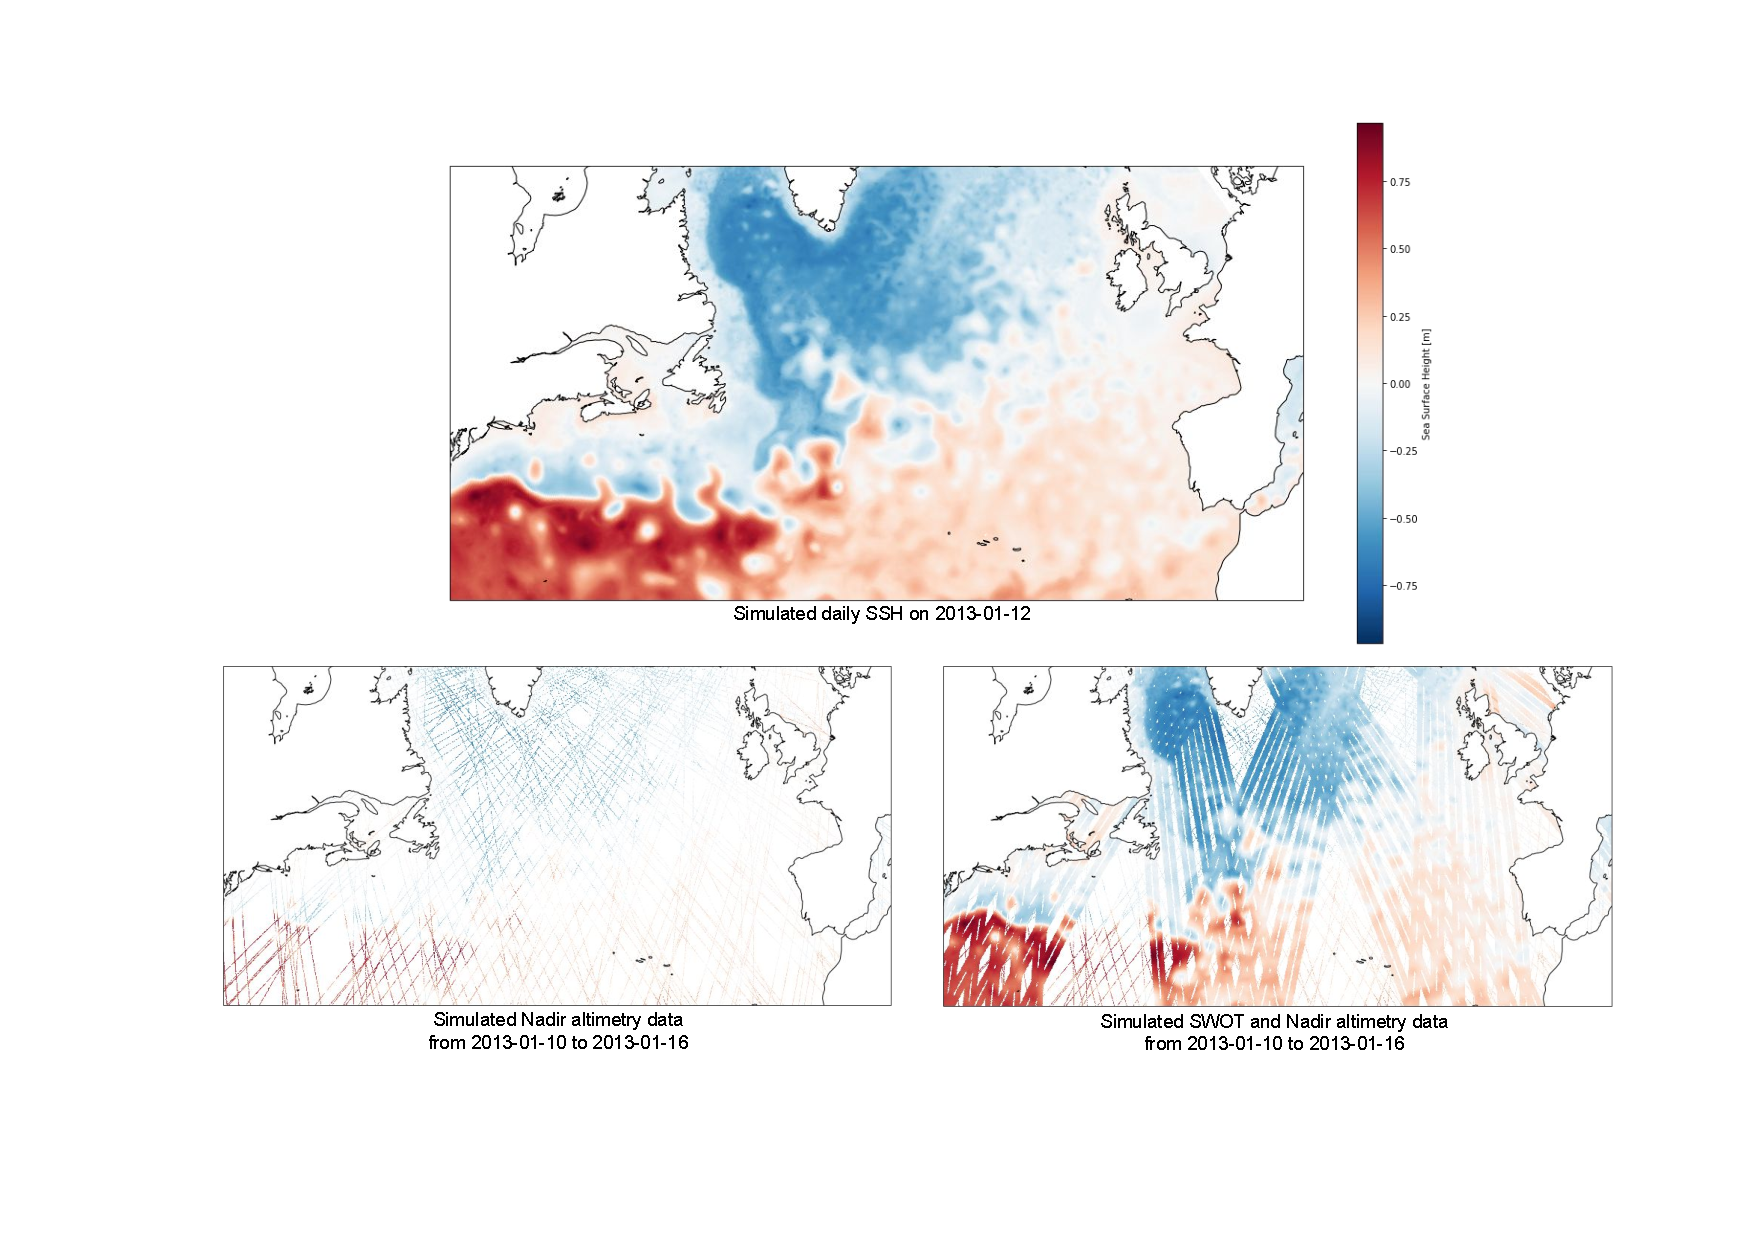
\includegraphics[width=21cm,clip,trim={1cm 3cm 0cm 2cm}]{Introduction/SSH_intro.pdf}}%
  % 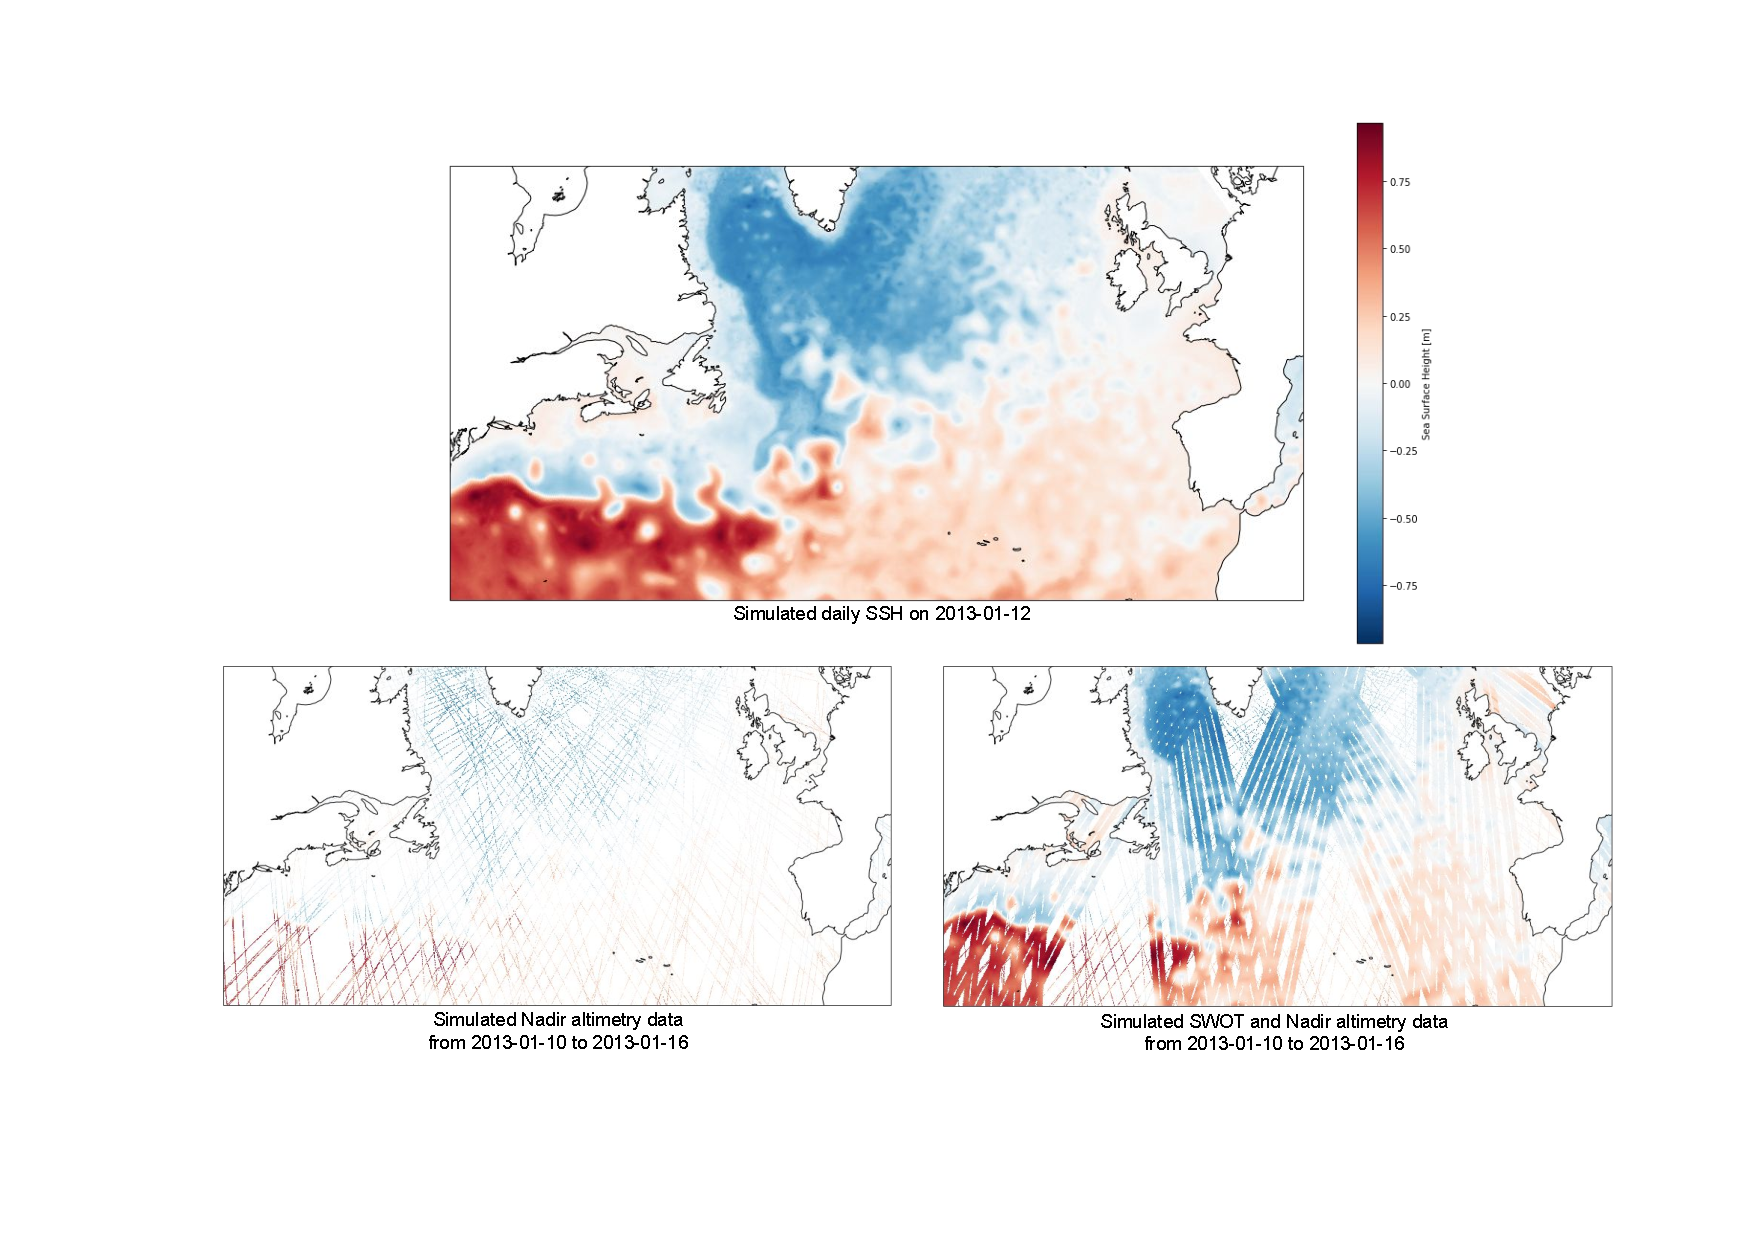
\includegraphics[width=19cm,center]{Introduction/SSH_intro.pdf}%
\centering    
    \caption{\textbf{Altimetry context.} The top figure display an example of average SSH over the north Atlantic from the NATL60 simulation. The bottom row illustrate the observational impact of the SWOT satellite.  }
    \label{fig:ssh_intro}
\end{figure}



  Finally we'll outline the structure of this manuscript. We'll present the altimetry use-cases and the deep learning methodological aspect considered in the third and fourth chapter. Finally, we'll introduce the scientific contribution of the OceanBench project which aims at facilitating collaboration between the ocean altimetry and deep learning communities.
  


  \section{Illustrative case and Key concepts: Graduating a thermometer}


\subsection*{Estimating temperature from observations}
\begin{figure}[h]
    \centering
        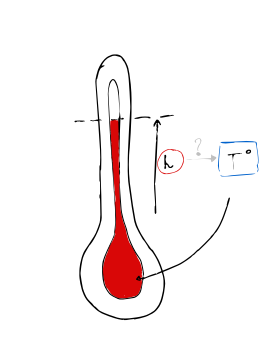
\includegraphics[clip, width=3cm]{Introduction/pics/therm_pb.png}
    \caption{\textbf{Thermometer Graduation problem illustration.} Given a simple liquid based thermometer, we aim at finding the matching between height of the liquid within the glass tube and temperature.}
    \label{fig:therm_calib}
\end{figure}

Let us consider a standard liquid based thermometer that consists of a liquid in a glass tube.
When interested in knowing the temperature, we observe the level of a thermometer.
In order to do so, someone had to graduate the thermometer. 
This seemingly simple action can be detailed in a two-step process, which involves the construction of a theoretical model and its calibration using real-world data.

The first step involves compiling theories and assumptions to construct a model linking the observed level and the actual temperature.
In this instance, based on our knowledge of fluid dilation in response to temperature, assuming the diameter of the tube is constant with height, we can propose the model that the level is linearly related with the temperature.
This model introduces two parameters: the slope and offset of our linear model that need to be ascertained.

The second step involves determining these parameters. This step requires some calibration data as inputs. They are traditionally obtained by immersing the thermometer in icing and boiling water to acquire the levels corresponding to 0°C and 100°C.
  Using those data points, a linear system can then be used to solve for the parameters. Which finally gives use our level-to-temperature relationship.


  The model we chose can have more or less independent parameters that need to be calibrated depending on the assumptions that were made.
  Interestingly, this introduce a relationship between the assumptions made and the amount of data required for calibration. For instance, a model with fewer assumptions demands more data. If we were to abandon the assumption of the thermometer tube's constant diameter, we would need to incorporate a parameterization of the tube diameter in our model. This addition creates more parameters and consequently demands additional data for calibration. Conversely, having access to more data can allow us to work with fewer assumptions. Suppose we possess a well-calibrated thermometer that can provide unlimited data points. In that case, we could reduce our assumptions to a minimum and rely heavily on empirical evidence, marking each thermometer graduation using data directly from our well-calibrated thermometer.

With these carefully calibrated graduations now etched onto our thermometer, we can use the liquid level as a convenient stand-in for the temperature. However, an important question remains: How can we assess the accuracy of our newly graduated thermometer?

\begin{figure}[h]
\centering
\begin{tabular}{ccc}

    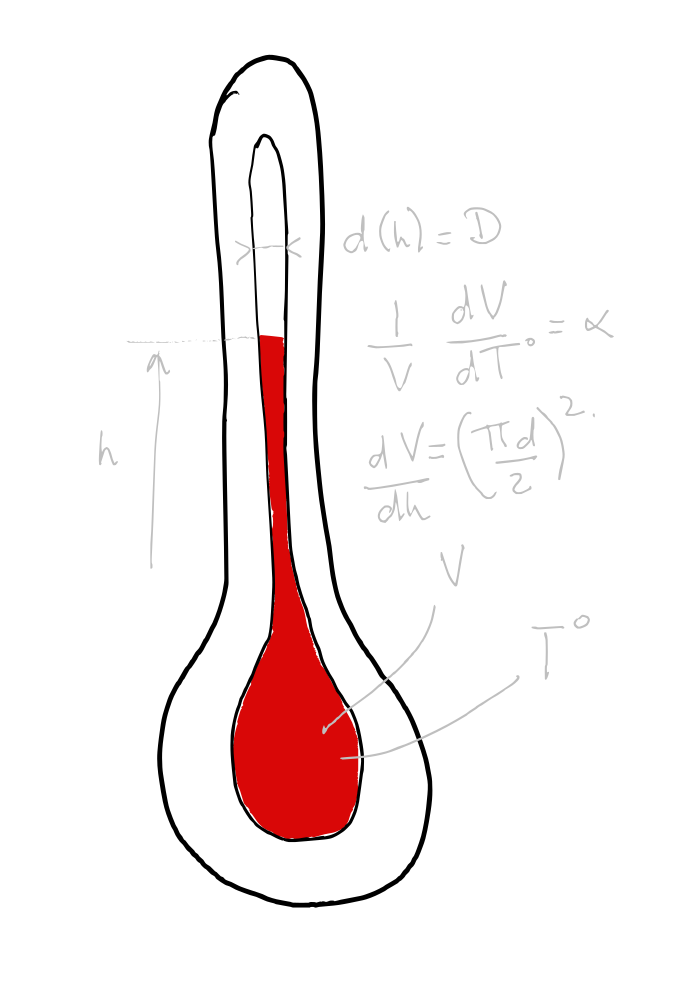
\includegraphics[clip, width=3cm, width=3cm]{Introduction/pics/therm_theroy.png} &   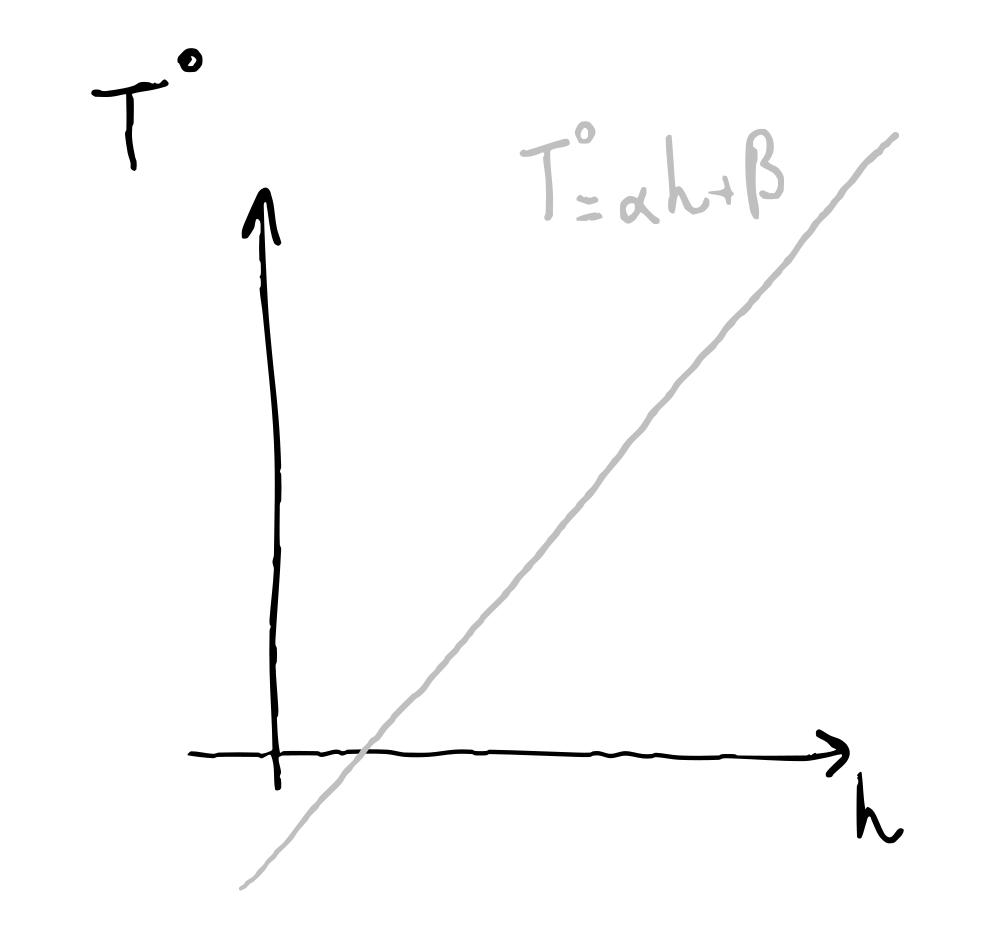
\includegraphics[clip, width=5cm]{Introduction/pics/therm_model.png}  &   \\   Assumptions & Model&\\ 
     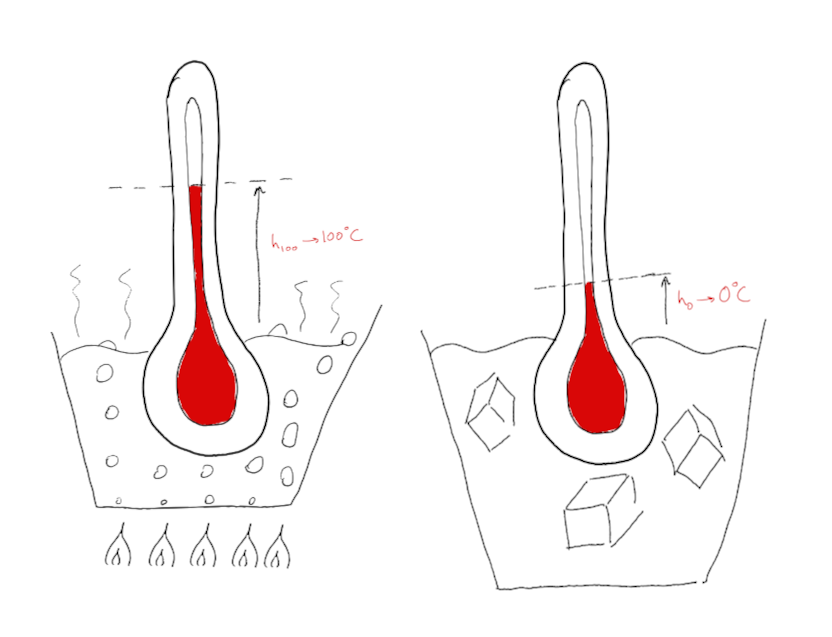
\includegraphics[clip, width=4cm, height=4cm, trim={2cm 1cm 2cm 2cm}]{Introduction/pics/therm_obs.png} &    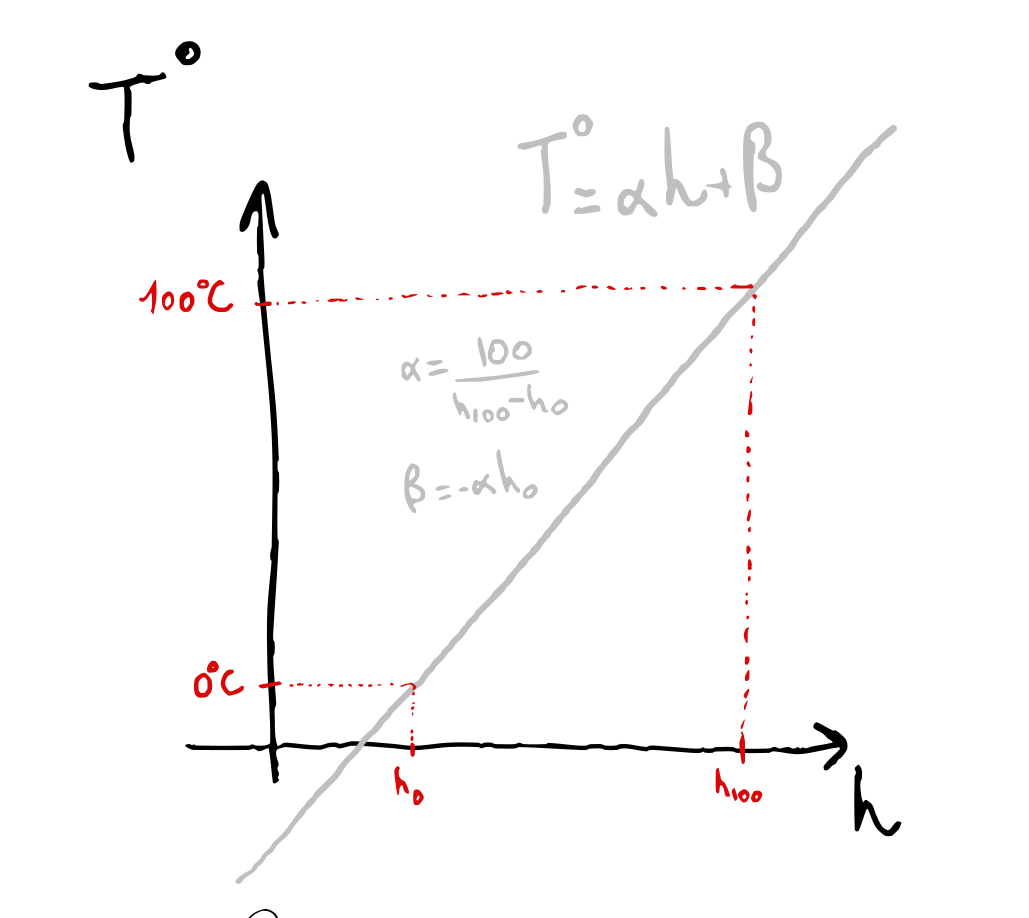
\includegraphics[clip, width=5cm]{Introduction/pics/therm_calib.png}   &  \\    Data & Calibration&\\
\end{tabular}

    \caption{\textbf{Mapping thermometer level to temperature.} The first step consists in compiling theoretical knowledge to determine a model of the level to temperature relationship. This model define the set of candidate graduations. The second step consists in leveraging data to chose the best candidate graduation through some calibration algorithm.}
    \label{fig:therm_mapping}
\end{figure}

\subsection*{Evaluation}

Without evaluation the use of our calibrated instrument would solely rely in the faith given to our mapping above.
However one may prefer quantifying the thermometers quality through metrics.
In our case the most intuitive metric for characterizing our thermometer's quality is be the precision of the graduations.
Each tick of our thermometer has a precision value, different aggregations of the individual values also constitute different metrics (bias versus variance for example)
In order to properly evaluate our calibrated instrument, we need to test it in conditions corresponding to its intended use. (testing it domestic thermometer 5 kilometers underwater would not give a relevant evaluation).

 To do so, let's explicit some assumptions made on what we expect from our thermometer.
  For example that it needs to "be accurate to the half of degree", "have response time under 10 minutes", "work between -30°C and 200°C" "work at a reasonable atmospheric pressure" etc...

Then we need data to measure the precision of our thermometer in a way that is representative of how we want our thermometer to behave. Using a trustworthy reference like a third-party well-graduated thermometer, we could compare the measurements of the reference with the one given by our solution.
  An example evaluation procedure could be to confront the measurements of the two instruments at different temperatures such as: in a freezer, in a fridge, at ambient room temperature and in an oven.

Using the procedure above, we can compute our precision metrics and assess if the quality of our thermometer is acceptable.
This exercise, raises some critical points about evaluation. The process relies on two components that require a deep understanding of the thermometer's intended use: a suitable choice of metrics and representative data.
If the metrics do not align with the intended use of the thermometer, the evaluation will be flawed. Similarly, if the data are not representative of the thermometer's intended use, the evaluation will also be flawed.
 Furthermore, the reliability of the reference thermometer is pivotal. If the reference thermometer is not well-graduated, the best of metrics will not be able to correctly evaluate our thermometer. 

It's also crucial to differentiate between calibration data, which is used to determine the graduation, and evaluation data, which is used to assess the graduation's quality.
A well-functioning thermometer should provide accurate temperature readings even for levels it wasn't calibrated on. Thus, evaluation data should differ from calibration data.
If we only measure precision at 0°C and 100°C, a thermometer that perfectly fits the calibration data would receive the highest metric, whatever the other graduation indicates.

\begin{figure}
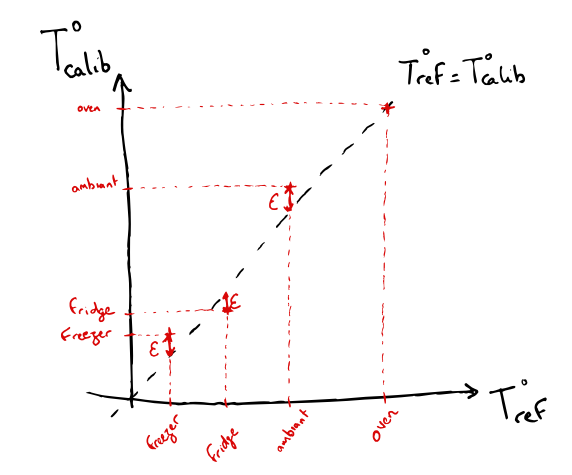
\includegraphics[clip, width=6cm]{Introduction/pics/errors.png}  
    \centering
    \caption{\textbf{Evaluation and errors.} Given some evaluation data and choice of metric, we can compute the errors associated with our graduation. $T^{\circ}_{calib}$ and $T^{\circ}_{ref}$ are respectively the temperatures given by our graduation and a reference well graduated thermometer}
    \label{fig:errors}
\end{figure}



 \subsection*{Sources of errors}


\begin{figure}
\begin{tabular}{c|c|c}
     \hspace{-.15\linewidth}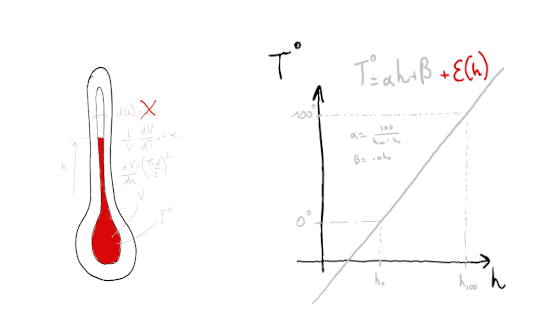
\includegraphics[width=.4\linewidth]{Introduction/pics/model_err_w_source.png}  &
     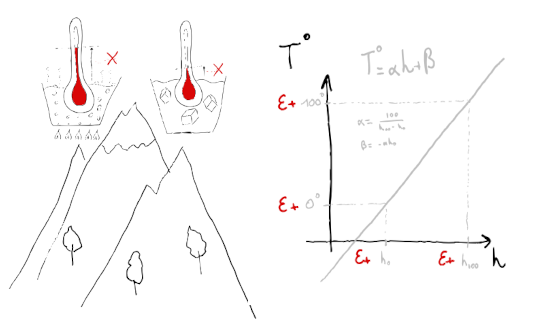
\includegraphics[width=.4\linewidth]{Introduction/pics/data_err_w_source.png} &
     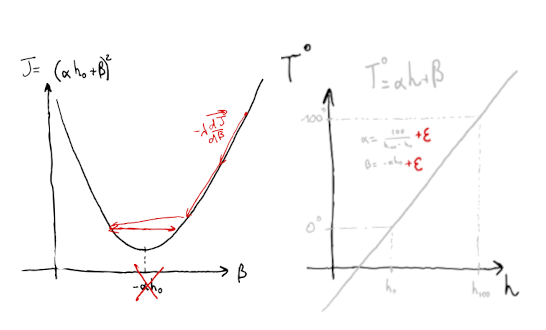
\includegraphics[width=.4\linewidth]{Introduction/pics/optim_err_w_source.png} \\
     \hspace{-.15\linewidth}Model &  Data &  Algorithm \\
\end{tabular}
    \centering
    \caption{\textbf{Illustration of the different sources of errors for the thermometer graduation.} From left to right: model errors result from erroneous assumptions about the system. Data errors result from inaccuracies in the calibration data and algorithmic errors result from a failure of the calibration algorithm to select the best candidate from the model.}
    \label{fig:err_sources}
\end{figure}
Given an evaluation procedure, the errors are the differences to the reference and can be attributed to three sources: the model, the data and the calibration algorithm.
 The model is a source of error if the assumptions made were inaccurate. For example if the diameter of the tube is not constant with height the linear relationship between level and temperature is not verified and will induce errors when interpreting the level.

 Even with perfect assumptions, noisy data can introduce errors in the calibration. If we interpreted our 0°C and 100°C in icing and boiling water at the top of a mountain with lower atmospheric pressure, we will have calibrated our parameters with erroneous measurements and the subsequent graduation of our thermometer will be inaccurate.

 Finally even with perfect assumptions and perfect data, the calibration algorithm used to find the solution's parameters can be a source of errors if it fails to find the optimal parameters. For example if we solve for the parameters with a gradient descent method, using a step size too big will prevent finding the exact parameters which will also results errors in the subsequent measurements.

In order to develop a graduation procedure, we need to take those sources of error into account. The graduation procedure choice will not only depend on the level-temperature relationship but on the whole relationship between calibration data to the final calibrated thermometer. We therefore need to incorporate in our reasoning how the calibration data was acquired, what is the best model to map the level to the temperature, and what is the best algorithm to find the optimal parameters of the model.


This example allows us to formulate a generic methodological framework.

\subsection*{Methodological framework}
In the process of finding a level-temperature relationship, we chose a model, a calibration algorithm, and had access to calibration data. Additionally, to evaluate our solution, we defined a metric and had access to evaluation data. Interestingly, these components can be specified at a higher level for finding and evaluating the graduation procedure itself, essentially creating a meta-level or "second order" problem.

The \textbf{Model}, in this second order scenario, combines different assumptions to determine the set of potential graduation procedures. 

The \textbf{Calibration Algorithm} is used to select the best graduation procedure. This could be as straightforward as testing different combinations and choosing the most effective one, or it could involve complex numerical optimization procedures to determine higher-level parameters.

The \textbf{Calibration Data}, at the second order, consists of graduation tasks with a method to assess the performance of candidate procedures. This allows the algorithm to select the best solution.

The \textbf{Evaluation Metric} should reflect the intended use of the graduation procedure, including the range of thermometers we plan to use this procedure for. A useful metric might be the precision of all the thermometers we aim to graduate using the proposed solution.

The \textbf{Evaluation Data} should be representative of the variety of intended uses. This means it should contain graduation tasks for a range of thermometers of interest. Additionally, we need a reference for these tasks to measure the precision of our solution.

By leveraging these five components, we can select the best graduation procedure, quantify its quality using the evaluation data, and use it to graduate new thermometers with confidence in the resulting graduated instrument. This parallels the problems of "Finding the level-temperature mapping" (which we refer to as the first order problem) and "Finding the graduation procedure" (the second order problem) and offers insights on where general purpose methodological tools can find applications.

Note that second order metrics can extend beyond the scope of the first order problem. These metrics could encompass aspects such as robustness to noise or the computational complexity of the graduation procedure. This means our evaluation of a graduation procedure not only includes how well it measures temperature, but also how well it handles uncertainties or computational burdens.

A second order solution takes first order calibration data as inputs, which contain observations of a specific thermometer and their corresponding temperatures, and outputs a first order solution: a tailored graduation for the thermometer represented in the data.

The second order problem also involves making decisions on parameters to select the best solution, which can take various forms. For instance, these parameters can be discrete choices between different assumptions, like whether to consider the thermometer's tube diameter as constant or not. The parameters can also denote choices between different first order algorithms like choosing a direct linear system inversion or a iterative optimization procedure. Lastly, these second order parameters can be constants in the level-temperature mappings or parameters of an optimization procedure, like step size. This shows that the parameters in the second order problem have a broad range of applicability, affecting both the details of the graduation procedure and how the procedure is chosen.

Finally, a critical note is that the data used to evaluate a solution at the second order level should still be separate from the calibration data. This principle holds true for the same reasons it applies to the first order problem - using distinct data sets helps to ensure that our solutions generalize well beyond the specific scenarios they were trained on.

\section{Applying the key notions to ocean altimetry}
\subsection*{Introducing space and time}
Our previous example implicitly solved the estimation problem of the liquid temperature within the thermometer at a single point in space and time.
However, we can extend the problem formulation to estimate a quantity over a spatial and temporal domain.
Given some observations $y$ defined on a spatio-temporal domain $\Omega_y$ we want to estimate a quantity of interest $u$ on a domain $\Omega_u$. We are therefore looking for a mapping $f$ that estimate $u$ from $y$
The process of determining $f$ can be detailed in two steps, first determining the set $\cal{F}$ such that $f \in \cal{F}$ by making some assumptions on $f$. Then determining the calibration algorithm $c$ that will use the calibration data $\cal{D}$ to select $f$ from $\cal{F}$
The evaluation of the solution rests on the choice of metrics $m$ and evaluation data $\cal{E}$

Solving this general problem requires considering the sampling pattern of the observations with respect to the target estimation domain.
Incomplete coverage will require the \textbf{model} to account for temporal and spatial relationship between $y$ values and $u$ as well as the spatio-temporal structure $u$.
These additional assumptions will require suitable \textbf{Calibration data and algorithm} and \textbf{Evaluation data and metrics} to be calibrated and evaluated.



\subsection*{Satellite altimetry}


The estimation of the sea surface height (SSH) given satellite altimetry data enters nicely in the methodological presented above.

  \begin{figure}[h]
      \centering
            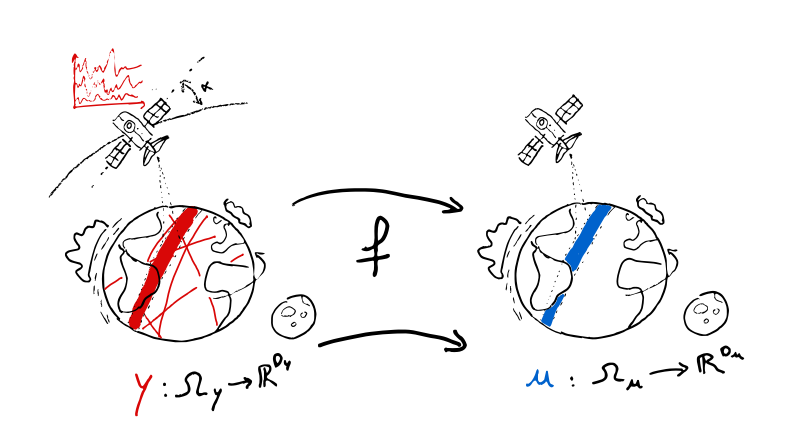
\includegraphics[width=\linewidth]{Introduction/pics/calib_task.png}    
      \caption{\textbf{SWOT calibration.} The left part illustrate the observed domain in red while the right part indicates the domain on which we aim at estimating the SSH.}
      \label{fig:calibration_task}
  \end{figure}
The calibration problem considered in this thesis consists in estimating the SSH measured by the KaRIN instrument by removing correlated error signals, using calibrated Nadir observations. The target estimation domain here is fully observed, however, some observations contains errors originating from the instrument acquisition process. The \textbf{model} for this problem includes assumptions about the processes that produce the errors. Note that some assumptions about the spatio-temporal structure of the SSH are also required here to relate the SSH on the KaRIN instrument to surrounding  NADIR altimeter measurements. The mapping problem below isolate this challenge more specifically.

\begin{figure}
    \centering
          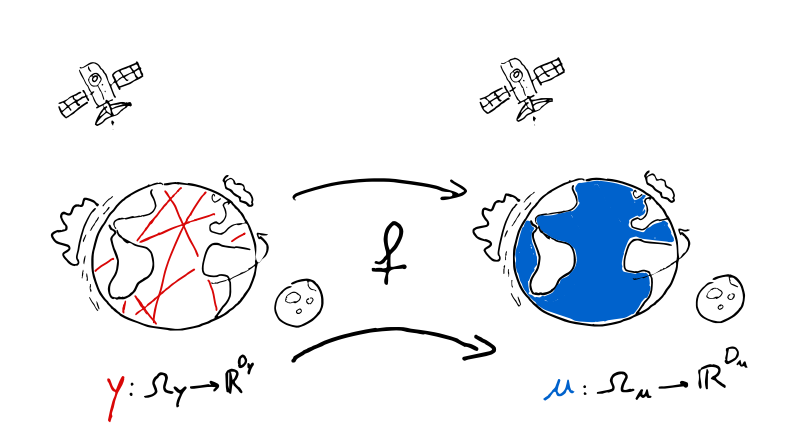
\includegraphics[width=\linewidth]{Introduction/pics/mapping_task.png}
    \caption{\textbf{Nadir Altimetry mapping.} The left part illustrate the observed domain in red while the right part indicates the domain on which we aim at estimating the SSH.}
    \label{fig:mapping_task}
\end{figure}
The altimetry mapping problem focuses on the spatial and temporal interpolation of NADIR altimetry data. Considering the observation as direct measurements of SSH, we aim at estimating daily maps over a delimited domain. The \textbf{model} for such a problem needs to take into account the dynamical structure of the ocean surface topography.

This manuscript, therefore, aims to explore the application of deep learning to these two observation problems. The first is estimating SSH from noisy SWOT observations, and the second is inferring the complete SSH field from partial measurements which we detail in the following two sections.
We give an overview of the next chapter the different \textbf{models} and \textbf{calibration algorithm} that have been developed for tackling these challenges.
  
In order to solve and evaluate solutions to these problems \textbf{Calibration and Evaluation data} are necessary. However, the SSH we aim to estimate is unknown on the target domain.
Two separate experimental setups are used to address this issue.
Observing System Experiments (OSE) \cite{hamonImpactMultipleAltimeter2019} constitute a framework for working directly with observations for calibrating and evaluating new methods.
For altimetry mapping for example, some satellite observations may be reserved for the interpolation process while others are employed to calibrate and evaluate the resulting map.
Observing System Simulation Experiments (OSSE)\cite{verrierAssessingImpactMultiple2017} use ocean models as well as simulated observing systems to create an controlled environment where simulated ocean quantities are known. For SWOT calibration, this includes simulating processes of the satellite movement such as roll oscillation that are sources of error signals\cite{EmpiricalCrossCalibrationCoherent}.
This peculiar data context is a critical factor when developing data-centric methods like deep learning.

% 

\section{Deep learning: opportunities and challenges}

\subsection*{Success stories in computer vision (CV) and natural language processing (NLP)}

In regard to the framework described above, deep learning brings forth \textbf{models}, such as neural networks, that are predicated on very weak assumptions. Their strength lies in the fact that, given sufficient parameters, they can approximate any function\cite{hornikMultilayerFeedforwardNetworks1989}. This leads to deep learning models defining vast parameter-space, consequently requiring substantial datasets and sophisticated optimization procedures to identify a good solution. These optimization procedures are akin to the \textbf{calibration algorithms}.

Deep learning \textbf{models} and \textbf{calibration algorithms} have advanced in tandem over the last decades.
Innovations in model architectures such as ResNet\cite{heDeepResidualLearning2016}, batch normalization\cite{ioffeBatchNormalizationAccelerating2015}, and in optimization procedures like Stochastic Gradient Descent (SGD)\cite{summaLargeScaleMachineLearning2011}, Adam\cite{kingmaAdamMethodStochastic2017}, and various learning rate schedules have consistently improved the calibration large models, therefore enabling the use of even larger neural networks. 

However, the fact that deep learning models can in theory approximate any function introduces a peculiar consideration which is that fitting exactly the calibration data gives you no guarantee on how the model will behave on unseen data.
Addressing this problem have motivated many innovations in regularization, architectures, initialization schemes and data augmentation techniques.
It has also standardized the practice of splitting the \textbf{calibration data} in two sets: \textbf{training} and \textbf{validation}.
The training set is used by the optimization procedure to search for the parameters whereas the validation set is used to assess the generalization on "unseen" data.

When looking at different application domain, the track records of deep learning in CV\cite{chaiDeepLearningComputer2021} and NLP\cite{brownLanguageModelsAre2020} are especially impressive. 
The tools brought by deep learning have managed to solve tasks that were previously unsolved.
Indeed the universality of deep learning models have brought a big leap forward in tasks such as natural image recognition or natural language generation which are very hard to model using theoretical knowledge.

Presented as such deep learning seems to provide universal tools.
However we would like to stress two factors that seem of great importance when looking at the contributions of deep learning in specific fields.
The first factor is quality and availability of data.
The creation of large, curated datasets, like ImageNet\cite{dengImageNetLargescaleHierarchical2009} in CV or ThePile\cite{gaoPile800GBDataset2020} in NLP have shown to dramatically expedite the development of novel approaches. 
The second factor is the design of informed architectural patterns that are particularly suited to the domain, leading to performance breakthroughs.
Examples of these include convolution techniques\cite{lecunHandwrittenDigitRecognition1989} and U-Net architectures\cite{ronnebergerUNetConvolutionalNetworks2015} in CV, and attention mechanisms\cite{vaswaniAttentionAllYou} in NLP. 
For the mapping and calibration challenges at hand in this thesis, the use of deep learning advances presents both opportunities and challenges that are introduced in next section.

\subsection*{Deep learning for ocean altimetry}

In deep learning, existing architectures used for video inpainting\cite{kimDeepVideoInpainting} and image denoising\cite{tianDeepLearningImage2020} solve tasks that are formally similar to altimetry mapping and calibration.
The universality of such models can potentially improve on existing methods by capturing processes relating to ocean dynamics and observations that are hard formulate formally.

Application of these models to altimetry however introduce some challenges related to the data.
The altimetry context do not provide access to the SSH state we want to estimate which raises questions concerning the calibration and evaluation of the model.
Indeed at the beginning of my thesis, the 4dVarNet neural mapping scheme was shown to surpass operational products for a usecase in the gulf stream area\cite{fabletENDTOENDPHYSICSINFORMEDREPRESENTATION2021}. However, this results had been calibrated and evaluated in an OSSE setup. 
This poses the question addressed in this manuscript is: \textit{How can deep learning approaches overcome the lack of true SSH for use on real altimetry?}
Furthermore, CV architectures have to some extent been iteratively validated and fitted on natural images.
The transfer to altimetry data and SSH fields and altimetry data is not trivial.
The sparse and irregular sampling pattern of altimeters  as well as the turbulent nature of the SSH may not be suited for classical CV architectures.

Furthermore, another factor that differentiate altimetry to previously mentioned fields is that classical methods already exist for solving the tasks considered. Existing methods use the available physical knowledge of ocean dynamics and observing systems. To some extent, this paints a less favorable setup for the potential of classical DL methods.
This raises another question we ask: \textit{How can specific altimetry knowledge be integrated in deep learning methodology?}


These studies demonstrate that altimetry analysis is fully dependent on domain expertise for both the data and evaluation contexts.
The development and evaluation of methods like the 4dVarNet relied heavily on prior efforts to standardize OSSE and OSE usecases in the form of data challenges\cite{ballarottaOceandatachallenges2020a_SSH_mapping_NATL60Material2020,ballarottaOceandatachallenges2021a_SSH_mapping_OSEMaterial2021}. These use-cases provided data access for machine learning practicioners as well as metrics relevant for ocean physicists. 
This raises the third question of this research: \textit{What is needed for a wide-spread adoption of deep learning tools in ocean observation sciences?}




\section{Thesis objectives and outline}

The following chapters of this thesis are organized as follows:

\textbf{Chapter 2} describes the main assumptions and methods that are formulated in current methods for altimetry mapping and calibration. This chapter aims at describing the existing \textbf{models} and \textbf{calibration algorithms} available in altimetry analysis as well as the related work in deep learning. A more detailed description of the neural network-based 4DVarNet framework and its applications will be presented since the contributions of this thesis make extensive use of this architecture.

\textbf{Chapter 3} propose a deep learning architecture for the calibration of correlated errors in SWOT data.
From an applicative standpoint, the flexibility of deep learning methodology opens the potential for capturing signals that are tricky to explicitly parameterize.
From a methodological perspective, this study shows how deep learning architectures can be tailored with assumptions on the instrument and its measurements.
More specifically, this is done by showing how the spectral specifities of the errors can be leveraged to design a efficient neural calibration scheme.
This study bypasses the challenges brought by the lack of ground-truthed dataset which is addressed in the following chapter.


\textbf{Chapter 4} tackles more specifically the data availability problem. It studies how neural mapping schemes can be applied to real data despite the lack of reference dataset.
It looks more specifically at the 4DVarNet framework which has been demonstrated in a simulated setup\cite{fabletENDTOENDPHYSICSINFORMEDREPRESENTATION2021} using simulated SSH for training and evaluation.
This chapter looks at the performance on real data of deep learning models trained on simulated data.
It shows how the extensive physical knowledge of the ocean dynamics can be leveraged to palliate the lack of ground-truthed dataset in altimetry through the use of numerical simulations for training.

\textbf{Chapter 5} considers the obstacles to better synergies between the ocean altimetry and deep learning communities.
Both fields are well established with accumulated knowledge, and best practices. 
As described in this chapter, deep learning brings powerful models and algorithms.
However the calibration and evaluation data as well as the metrics can only be sensibly designed by an domain expert. 
We propose OceanBench, an interface in the form of a software suite of tools.
Oceanbench aims at empowering domain experts to easily design altimetry problems of interests and qualifying them with relevant metrics. 
It then provides machine learning practitioners access to the necessary data as well as suited utilities for training and evaluating learning based methods.

\textbf{Chapter 6} discusses and concludes on the research presented in this manuscript. We summarize the main objectives and results in previous chapters as well as proposing some future avenues of research.


\addcontentsline{toc}{section}{Bibliography}
\putbib[./Introduction/Intro-Biblio.bib]
\end{bibunit}

